\documentclass[mathserif]{beamer}
\usetheme{Boadilla}
%\usepackage[francais]{babel}
\usepackage[utf8]{inputenc} % Uses the utf8 input encoding
\usepackage[T1]{fontenc} % Use 8-bit encoding that has 256 glyphs

\usepackage[nomath]{kpfonts}
\usepackage{eulervm}
%\usepackage{default}

\usepackage{amsthm}
\usepackage{amssymb}
\usepackage{xparse}
\usepackage{thmtools}
\usepackage{stackrel}

%shortcuts
\newcommand{\R}{\mathbb{R}}
\newcommand{\C}{\mathbb{C}}
\newcommand{\Z}{\mathbb{Z}}
\newcommand{\N}{\mathbb{N}}
\newcommand{\fii}{\varphi}
\newcommand{\dd}{\mathrm{d}}
\newcommand{\CP}{\mathbb{CP}}
\renewcommand{\S}{\mathbb{S}}
\DeclareMathOperator{\Sp}{Sp}
\DeclareMathOperator{\tr}{tr}
\DeclareMathOperator{\dist}{dist}

% theorems configuration

\makeatletter
\newtheoremstyle{indented}
{7pt} %vertical space before
{7pt} % vertical space after
{} %{\addtolength{\@totalleftmargin}{2.5em}
	%\addtolength{\linewidth}{-3.5em}
	%\parshape 1 3.5em \linewidth} %body font
{1.5em} %indent
{\bfseries} %header font
{.} %punctuation
{.5em} %horizontal space after header
{} %header specification

\theoremstyle{definition}

\newtheorem{defn}{Définition}[section]

\theoremstyle{plain}
%\newtheorem*{theorem*}{Theorem}

\newtheorem{thm}{Théorème}

\renewcommand{\thetheorem}{\Alph{theorem}}
\newenvironment{preuve}{
	\noindent \textbf{Proof. }}{\hfill $\square$\medskip\par}

\newtheorem{exemple}[defn]{Example}
\newtheorem{prop}[defn]{Proposition}
\newtheorem{corr}[defn]{Corollary}
\newtheorem{por}[defn]{Porisme}
\newtheorem{ex}[defn]{Example}
\newtheorem{lem}[defn]{Lemma}
\newtheorem{conj}{Conjecture}
\newtheorem{ax}{Axiom}  %Axioms have their own numerotation

\theoremstyle{definition}
\newtheorem{rem}[defn]{Remark} %remarks are not indented
\newtheorem{rems}[defn]{Remarks}

%--------------
% Mise en page mathématique
%--------------
\addtolength{\jot}{.2em}


\title{Szeg\H{o} kernels and Toeplitz operators}
\author{Alix Deleporte}
\institute{MSRI}

\AtBeginSection
{
	\begin{frame}
		\frametitle{Plan}
		\tableofcontents[currentsection]
	\end{frame}
	
}

\newcommand{\spline}{\hline}
\renewcommand{\arraystretch}{1.3}
\begin{document}
\begin{frame}
	\titlepage
\end{frame}

\section{Toeplitz operators on $\C^n$}
\begin{frame}
  \frametitle{Quantization of the harmonic oscillator}
  Quantization: associate {\bf classical dynamics} (driven by
  real-valued functions) with {\bf self-adjoint operators}.

  \uncover<2->{\begin{center}
    \begin{tabular}{ccc}
      classical & $\rightsquigarrow$ & quantum\\\hline
      \uncover<3->{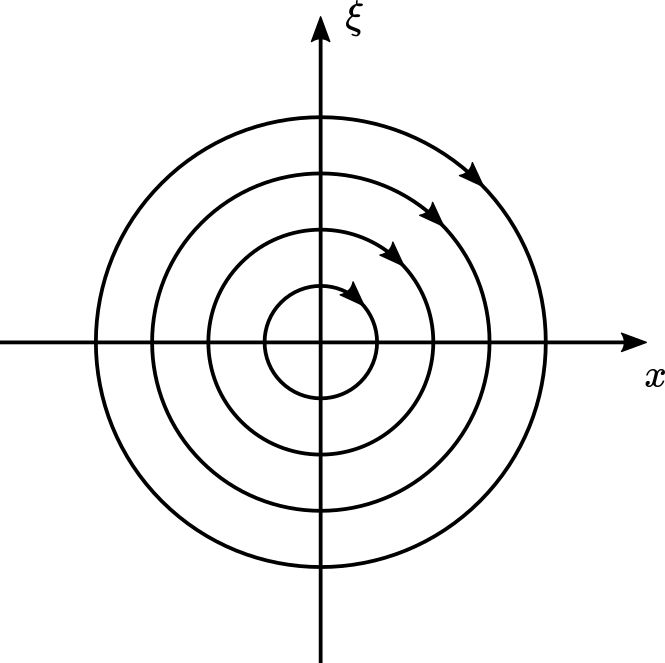
\includegraphics[scale=0.2]{harm_phase.png}}&&\uncover<6>{\begin{minipage}{}
        ???\\
        \vspace{7em}\end{minipage}\vspace{-3em}}\\
      \uncover<4->{{\tiny $x(t)=\sqrt{x_0^2+\xi_0^2}\cos\left[t-\arctan\left(\frac{\xi_0}{x_0}\right)\right]$}}& &\uncover<5->{$H_n(x)e^{-\frac{x^2}{2}}$}
    \end{tabular}
  \end{center}}
\end{frame}

\begin{frame}
  \frametitle{Bargmann spaces}
  \begin{itemize}
  \item Original idea: express Quantum Mechanics directly in phase
    space.
  \uncover<2->{\item The standard $L^2(\R^n)$ is replaced with the \emph{Bargmann
      space}, with parameter $N>0$ (think of $N=\hbar^{-1}$):
$$B_N=L^2(\C^n)\cap\left\{e^{-\frac N2 |\cdot|^2}f,\,f\text{ is
  holomorphic on $\C^n$}\right\}.$$}\vspace{-2em}
  \uncover<3>{\item This is a closed subspace of $L^2(\C^n)$, with reproducing
    kernel
$$\Pi_N(x,y)=\left(\frac N{\pi}\right)^n\exp\left(-\cfrac N2
  |x-y|^2+iN\Im(x\cdot \overline{y})\right).$$}
  \end{itemize}
\vspace{-1em}
\small{[1] Bargmann, V. Comm. Pure Appl. Math. 14, no. 3 (1961): 187–214.}

\end{frame}

\begin{frame}
  \frametitle{Szeg\H{o} kernel}
  Hilbert basis indexed by $\N^{n}$:

$$e_{\nu}=\uncover<2->{\cfrac{N^{|\nu|}}{\nu_1!\nu_2!\ldots\nu_n!}}\,z^{\nu}e^{-\frac{N|z|^2}{2}}.$$

\uncover<3>{From there one recovers $\Pi_N$ with
$$\Pi_N(x,y)=\sum_{\nu\in \N^n} e_{\nu}(x)\overline{e_{\nu}}(y).$$

The Szeg\H{o} kernel decays exponentially fast away from the diagonal.
}
\end{frame}

\begin{frame}
  \frametitle{Quantum harmonic oscillator}
  \begin{itemize}
  \item Let us quantize $x^2+\xi^2=|z|^2=\overline{z}z$.
  \item<2-> $z$ acts by multiplication.
  \item<3-> $\overline{z}$ acts as its adjoint; it acts as
    $N^{-1}\partial+\frac 12 \overline{z}=\mathfrak{d}_N$.
  \item<4-> {\bf ordering choice}: $Op(x^2+\xi^2)=\mathfrak{d}_Nz$.
  \item<5-> $\langle u,\mathfrak{d}_Nzv\rangle=\langle
    zu,zv\rangle=\langle u,|z|^2v\rangle$.
  \item<6> Spectrum: $N^{-1}\N$; eigenfunctions: monomials. 
  \end{itemize}
\end{frame}

\begin{frame}
  \frametitle{Toeplitz quantization}
  Let $f\in C^{\infty}(\C^n,\C)$ bounded. The Toeplitz operator associated
  with $f$ is the bounded operator
\begin{center}
\begin{array}{rcl}
 		T_N(f):B_N(\C^n)&\mapsto & B_N(\C^n)\\
		u& \mapsto& \uncover<2->{\Pi_N(}fu\uncover<2->{)}.
 		\end{array}
\end{center}

\uncover<3->{If $f$ has polynomial growth then $T_N(f)$ is an unbounded operator
with dense domain.}
\uncover<4>{\begin{itemize}
\item If $f$ is real-valued then $T_N(f)$ is ess. self-adjoint.
\item If moreover $f\geq 0$ then $T_N(f)\geq 0$.
\end{itemize}}
\end{frame}

\begin{frame}
  \frametitle{Composition of Toeplitz operators}
  \begin{itemize}
  \item Recipe: \[T_N(z\mapsto \overline{z}^{\alpha}z^{\beta})=\mathfrak{d}_N^{\alpha}z^{\beta}.\]

\uncover<2->{\item The Toepliz quantization is \emph{anti-Wick}: if $f$ is
  anti-holomorphic and $h$ is holomorphic then
\[T_N(fgh)=T_N(f)T_N(g)T_N(h).\]}
\uncover<3>{\vspace{-1.5em}\item More generally, composition yields a formal series:
\[T_N(f)T_N(g)=T_N\left(fg+N^{-1}C_1(f,g)+N^{-2}C_2(f,g)+\cdots\right).\]

$C_j$ is a bidifferential operator of total order $2j$.}
\end{itemize}
\end{frame}

\begin{frame}
  \frametitle{Toeplitz operators versus $\Psi$DOs}
  \begin{itemize}
  \item The Bargmann transform $\mathcal{B}_N$ conjugates $B_N$ and
    $L^2(\R^n)$.
  \uncover<2->{\item It is related to the FBI
    transform.}
  \uncover<3->{
  \item With $g_N=(N/\pi)^ne^{-N|z|^2}$ one has
    \[
      \mathcal{B}_N^{-1}T_N(f)\mathcal{B}_N=Op_W^{N^{-1}}(f*g_N).
    \]\vspace{-2em}}
\uncover<4->{\item Formal equivalence between Toeplitz and $\Psi$DO
  calculus.}
\uncover<5>{\item Toeplitz quantization is formulated {\bf directly in
  phase space}, and {\bf positive}.}

  \end{itemize}
\end{frame}

\section{Toeplitz operators on compact manifolds}
\begin{frame}\frametitle{Generalized Bargmann spaces}
  \begin{itemize}
    \item Changing the positive quadratic weight in the Bargmann space:
  \[
    B_N^{\psi}=\left\{f\in L^2(\C^n), e^{-N\psi}f \text{ is
        holomorphic}\right\}
  \]
  is another closed subspace of $L^2$.

  \item<2-> Commutator of Toeplitz operators $\rightsquigarrow$
    squeezed symplectic form given by
    $\partial\overline{\partial}\psi$.
    
  \item<3-> Infinitesimal model for the case where $\psi$ is an
    arbitrary strongly pseudoconvex function $\Leftrightarrow$ arbitrary
    symplectic form on $\R^{2n}$.
      \item<4> Note: one cannot simplify both symplectic and complex
          structure at the same time!
      \end{itemize}
    \end{frame}

\begin{frame}
  \frametitle{Hardy spaces and Szeg\H{o} kernel}
  \begin{itemize}
  \item Geometrical setting: compact K\"ahler manifold $M$.\\
    \begin{minipage}{0.37\linewidth}\begin{itemize}
    \item Symplectic form
    \item Complex structure
    \end{itemize}
\end{minipage}
\uncover<2->{\begin{minipage}{0.52\linewidth}

$\biggl\}$ Compatibility condition
\end{minipage}}
\uncover<3->{\item Complex line bundle $L\to M$ with curvature
  $-i\omega$: glue together pieces of Bargmann spaces in holomorphic charts.}
\uncover<4->{\item Hardy space $H_N(M,L)$ of holomorphic sections of $L^{\otimes N}$.}
\uncover<5->{\item Szeg\H{o} projector $S_N:L^2(M,L^{\otimes N})\to H_N(M,L).$}
  \end{itemize}

\vspace{5em}
\small{[2] Woodhouse, N. Geometric Quantization. Oxford University Press, 1997.}
\end{frame}

\begin{frame}
  \frametitle{Algebra of Toeplitz operators}
  \begin{itemize}
  \item The Szeg\H{o} kernel $S_N$ has a full expansion near the
    diagonal, and decays far from it.
  \uncover<2->{\item Indeed $S_N$ can be seen as the $N$-th Fourier mode of a
    Fourier Integral Operator with complex phase; the critical set is
    the diagonal.}
\uncover<3->{\item The dominant term is always $\Pi_N$.}
  \uncover<4>{\item Toeplitz operators form a $C^{*}$-algebra as previously.} 
  \end{itemize}
\vspace{2em}

\small{[3] Boutet de Monvel, L, Sjöstrand, J. Journées EDP 34–35 (1975): 123–64.

[4] Charles, L. Comm. Math. Phys. 239, no. 1–2 (2003): 1–28.

[5] Berman, R., Berndtsson, B., Sjöstrand, J.,  Arkiv För Matematik
46, no. 2 (2008).

{\bf [6] Deleporte, A. preprint arXiv:1812.07202}
}

 

\end{frame}

\begin{frame}
  \frametitle{An example: the 2D sphere}
  Here $M=\mathbb{S}^2$. In the stereographic projection, $L$
  corresponds to the weight $z\mapsto \frac{1}{1+|z|^2},$ so
  that \begin{align*}H_N(M,L)&\simeq \left\{f\text{ holomorphic in
                               $\C$},\,\int_{\C}\cfrac{|f|^2}{(1+|z|^2)^{N+2}}<\infty\right\}\\
                             &=\C_N[X].\end{align*}
\uncover<2>{In the canonical basis $\binom{N}{k}^{-\frac 12}X^k$, the Toeplitz
quantization of the three base coordinates on $\mathbb{S}^2$ are the Spin
matrices with spin $S=\frac {N-1}2$.}
\end{frame}



\section{Melin estimate}
\begin{frame}
  \frametitle{Characteristic value}
  Can one improve the lower bound $f\geq 0\Rightarrow T_N(f)\geq 0$ ?
  \begin{itemize}
  \item If $q$ is a quadratic form in $\C^n$, the minimal eigenvalue
    of $T_N(q)$ is $N^{-1}\mu(q)$ with $$\mu(q)=N^{-1}(Tr^+(q)+\frac
    12 \tr(q)).$$
  \uncover<2>{\item Here, up to a
    symplectomorphism, $$q=\sum_{i=1}^{r}\lambda_i(q_i^2+p_i^2)+\sum_{i=r+1}^{r+r'}p_i^2,$$
    so $$Tr^+(q)=\sum_{i=1}^r\lambda_i.$$
}

\end{itemize}
\end{frame}

\begin{frame}
  \frametitle{Estimates on the first eigenfunction}
  \begin{enumerate}
  \item<1-> {\bf Upper estimate}: try states localised near a point
    $x$ where $f$ is minimal:
    contribution $\min(f)+N^{-1}\mu(\Hess(f)(x))+O(N^{-2})$.
  \item<2-> Corresponding lower bound for {\bf states localised near a
      point}.
  \item<3-> Proof in three steps:
    \begin{itemize}
    \item Small energy eigenfunctions localize where $f$ is minimal.
    \item Cut into pieces of size $N^{-\frac 12+\epsilon}$ {\bf
        corresponding to the eigenfunction} (see next slide)
      \item Apply the lower bound on each piece.
    \end{itemize}

  \end{enumerate}
\end{frame}
\begin{frame}
  \frametitle{A cutting lemma}
  A function cannot be too large everywhere!
\vfill 
  Example: given $t<a$ and $u:\S^1\to \R$, then $\S^1$ can be cut into pieces $U_j$ of size
  between $a$ and $2a$, with overlap $t$, such that
  \[
    \sum_{i,j}\int_{U_i\cap U_j}|u|\leq
    C\frac{t}{a}\sum_i\int_{U_i}|u|.
    \]
  \end{frame}

  \begin{frame}
\frametitle{Melin estimate}
\begin{theorem}
    If $f\in C^{\infty}(M,\R)$ and if $\mu_{inf}$ is the infimum of $\mu$ over all
    minimal points, then $$T_N(f)\geq \min(f)+N^{-1}\mu_{inf}+N^{-1-\epsilon}.$$
  \end{theorem}
  
\vspace{7em}
\small{
  [8] Melin, A. Arkiv För Matematik 9, no. 1 (1971): 117–140
  
{\bf [9] Deleporte, A. Comm. Math. Phys (accepted)}
}

\end{frame}

\begin{frame}
  \frametitle{Consequence: localization of the ground state}
  \begin{minipage}[l]{0.3\linewidth}
    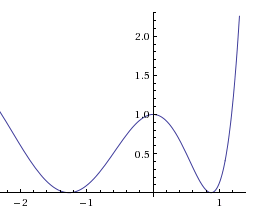
\includegraphics[width=\linewidth]{wells.png}
  \end{minipage}
  \begin{minipage}[r]{0.65\linewidth}
    What can be said about the ground state, using the Melin estimate?
    
    \uncover<2->{
      \begin{thm}
        The eigenvectors of minimal eigenvalue concentrate only on
        ``minimal'' points. Eigenvectors and eigenvalues have an
        asymptotical expansion in powers of $N^{-\frac 12}$.
      \end{thm}
    }

    \uncover<3>{What is minimized ? The $\mu$ of the Hessian at this
      point.}
  \end{minipage}

  \vspace{2em}

\small{{\bfseries [9] Deleporte, A., Journal of Spectral Theory
    (accepted)}}
\end{frame}





\end{document}
%%% Local Variables:
%%% mode: latex
%%% TeX-master: t
%%% End:
